\documentclass{standalone}
\usepackage{tikz}
\usetikzlibrary{patterns, positioning}

\begin{document}
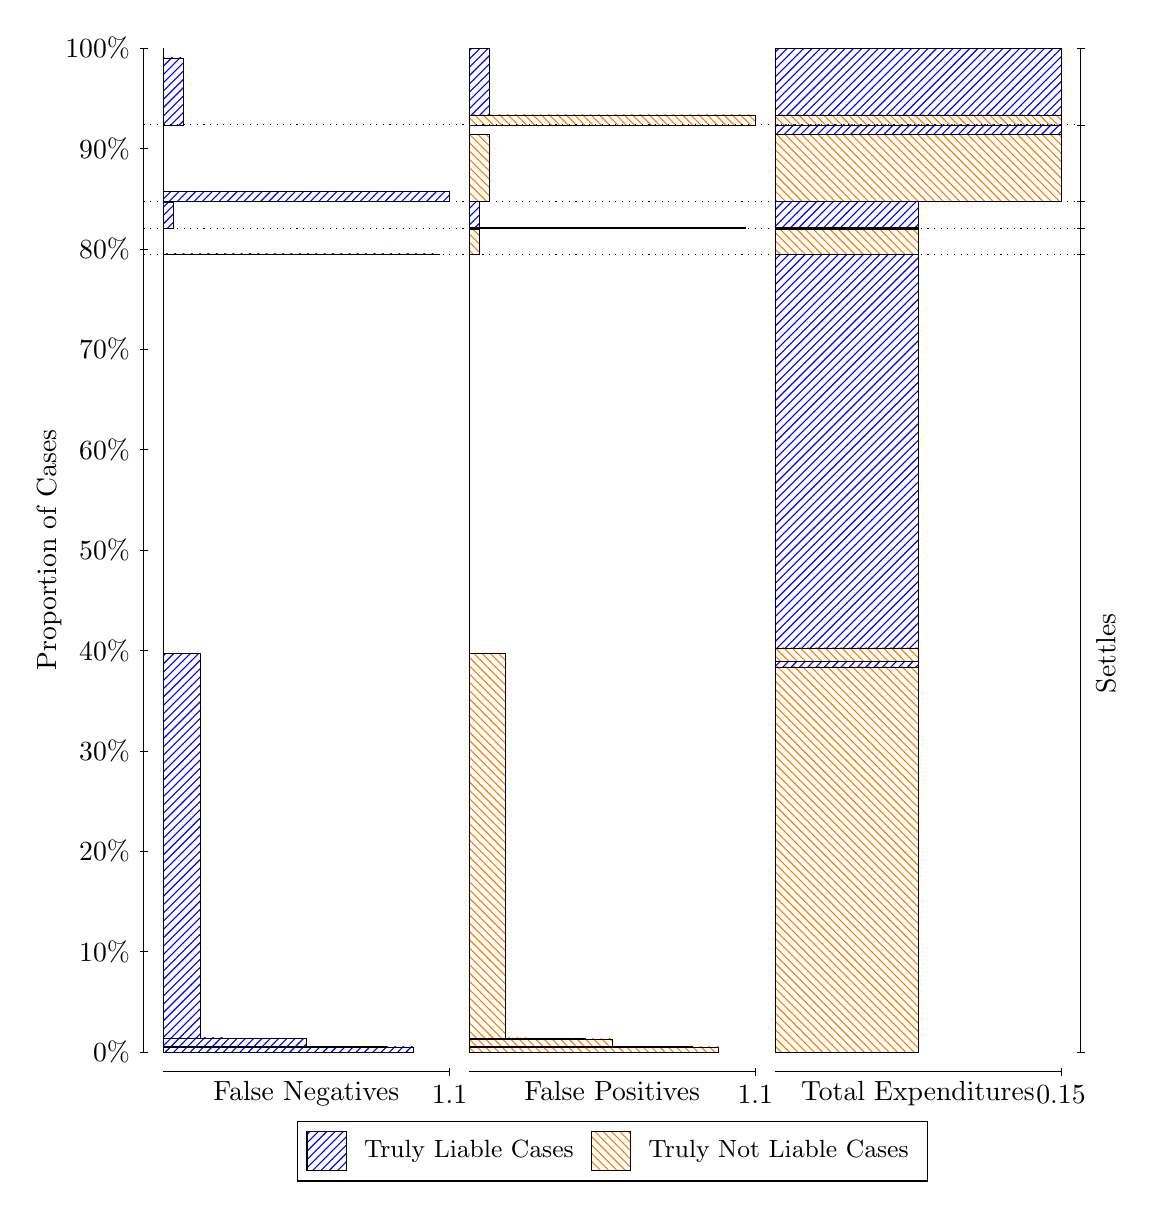
\begin{tikzpicture}
\draw[black, very thin] (1.5,1.75) -- (1.5,14.5);
\node[rotate=90, anchor=center] at (0.3, 8.125) {Proportion of Cases};
\draw[black, very thin] (1.45,1.75) -- (1.55,1.75);
\node[anchor=east] at (1.45, 1.75) {0\%};
\draw[black, very thin] (1.45,3.025) -- (1.55,3.025);
\node[anchor=east] at (1.45, 3.025) {10\%};
\draw[black, very thin] (1.45,4.3) -- (1.55,4.3);
\node[anchor=east] at (1.45, 4.3) {20\%};
\draw[black, very thin] (1.45,5.575) -- (1.55,5.575);
\node[anchor=east] at (1.45, 5.575) {30\%};
\draw[black, very thin] (1.45,6.85) -- (1.55,6.85);
\node[anchor=east] at (1.45, 6.85) {40\%};
\draw[black, very thin] (1.45,8.125) -- (1.55,8.125);
\node[anchor=east] at (1.45, 8.125) {50\%};
\draw[black, very thin] (1.45,9.4) -- (1.55,9.4);
\node[anchor=east] at (1.45, 9.4) {60\%};
\draw[black, very thin] (1.45,10.675) -- (1.55,10.675);
\node[anchor=east] at (1.45, 10.675) {70\%};
\draw[black, very thin] (1.45,11.95) -- (1.55,11.95);
\node[anchor=east] at (1.45, 11.95) {80\%};
\draw[black, very thin] (1.45,13.225) -- (1.55,13.225);
\node[anchor=east] at (1.45, 13.225) {90\%};
\draw[black, very thin] (1.45,14.5) -- (1.55,14.5);
\node[anchor=east] at (1.45, 14.5) {100\%};

\draw[black, very thin] (13.4,1.75) -- (13.4,14.5);
\draw[black, very thin] (13.35,1.75) -- (13.45,1.75);
\node[anchor=west] at (13.35, 1.75) {};
\draw[black, very thin] (13.35,11.878) -- (13.45,11.878);
\node[anchor=west] at (13.35, 11.878) {};
\draw[black, very thin] (13.35,12.211) -- (13.45,12.211);
\node[anchor=west] at (13.35, 12.211) {};
\draw[black, very thin] (13.35,12.55) -- (13.45,12.55);
\node[anchor=west] at (13.35, 12.55) {};
\draw[black, very thin] (13.35,13.525) -- (13.45,13.525);
\node[anchor=west] at (13.35, 13.525) {};
\draw[black, very thin] (13.35,14.5) -- (13.45,14.5);
\node[anchor=west] at (13.35, 14.5) {};

\draw[black, very thin, pattern color=blue, pattern=north east lines] (1.75,1.75) rectangle (4.9186,1.8139);
\draw[black, very thin, pattern color=blue, pattern=north east lines] (1.75,1.8139) rectangle (4.5806,1.8161);
\draw[black, very thin, pattern color=blue, pattern=north east lines] (1.75,1.8161) rectangle (4.2426,1.8184);
\draw[black, very thin, pattern color=blue, pattern=north east lines] (1.75,1.8184) rectangle (3.9047,1.8207);
\draw[black, very thin, pattern color=blue, pattern=north east lines] (1.75,1.8207) rectangle (3.5667,1.918);
\draw[black, very thin, pattern color=blue, pattern=north east lines] (1.75,1.918) rectangle (3.2287,1.9216);
\draw[black, very thin, pattern color=blue, pattern=north east lines] (1.75,1.9216) rectangle (2.8907,1.9254);
\draw[black, very thin, pattern color=blue, pattern=north east lines] (1.75,1.9254) rectangle (2.5527,1.9291);
\draw[black, very thin, pattern color=blue, pattern=north east lines] (1.75,1.9291) rectangle (2.2147,6.8113);
\draw[black, very thin, pattern color=orange, pattern=north west lines] (1.75,6.8113) rectangle (1.75,11.878);
\draw[black, very thin, pattern color=blue, pattern=north east lines] (1.75,11.878) rectangle (5.2566,11.887);
\draw[black, very thin, pattern color=orange, pattern=north west lines] (1.75,11.887) rectangle (1.75,12.211);
\draw[black, very thin, pattern color=blue, pattern=north east lines] (1.75,12.211) rectangle (1.8767,12.54);
\draw[black, very thin, pattern color=orange, pattern=north west lines] (1.75,12.54) rectangle (1.75,12.55);
\draw[black, very thin, pattern color=blue, pattern=north east lines] (1.75,12.55) rectangle (5.3833,12.676);
\draw[black, very thin, pattern color=orange, pattern=north west lines] (1.75,12.676) rectangle (1.75,13.525);
\draw[black, very thin, pattern color=blue, pattern=north east lines] (1.75,13.525) rectangle (2.0035,14.374);
\draw[black, very thin, pattern color=orange, pattern=north west lines] (1.75,14.374) rectangle (1.75,14.5);
\draw[black, very thin, pattern color=orange, pattern=north west lines] (5.6333,1.75) rectangle (8.8019,1.8139);
\draw[black, very thin, pattern color=orange, pattern=north west lines] (5.6333,1.8139) rectangle (8.464,1.8161);
\draw[black, very thin, pattern color=orange, pattern=north west lines] (5.6333,1.8161) rectangle (8.126,1.8183);
\draw[black, very thin, pattern color=orange, pattern=north west lines] (5.6333,1.8183) rectangle (7.788,1.8204);
\draw[black, very thin, pattern color=orange, pattern=north west lines] (5.6333,1.8204) rectangle (7.45,1.9176);
\draw[black, very thin, pattern color=orange, pattern=north west lines] (5.6333,1.9176) rectangle (7.112,1.9177);
\draw[black, very thin, pattern color=orange, pattern=north west lines] (5.6333,1.9177) rectangle (7.112,1.9216);
\draw[black, very thin, pattern color=orange, pattern=north west lines] (5.6333,1.9216) rectangle (6.774,1.9255);
\draw[black, very thin, pattern color=orange, pattern=north west lines] (5.6333,1.9255) rectangle (6.436,1.9292);
\draw[black, very thin, pattern color=orange, pattern=north west lines] (5.6333,1.9292) rectangle (6.0981,6.8166);
\draw[black, very thin, pattern color=blue, pattern=north east lines] (5.6333,6.8166) rectangle (5.6333,11.878);
\draw[black, very thin, pattern color=orange, pattern=north west lines] (5.6333,11.878) rectangle (5.7601,12.202);
\draw[black, very thin, pattern color=blue, pattern=north east lines] (5.6333,12.202) rectangle (5.6333,12.211);
\draw[black, very thin, pattern color=orange, pattern=north west lines] (5.6333,12.211) rectangle (9.1399,12.22);
\draw[black, very thin, pattern color=blue, pattern=north east lines] (5.6333,12.22) rectangle (5.7601,12.55);
\draw[black, very thin, pattern color=orange, pattern=north west lines] (5.6333,12.55) rectangle (5.8868,13.399);
\draw[black, very thin, pattern color=blue, pattern=north east lines] (5.6333,13.399) rectangle (5.6333,13.525);
\draw[black, very thin, pattern color=orange, pattern=north west lines] (5.6333,13.525) rectangle (9.2667,13.651);
\draw[black, very thin, pattern color=blue, pattern=north east lines] (5.6333,13.651) rectangle (5.8868,14.5);
\draw[black, very thin, pattern color=orange, pattern=north west lines] (9.5167,1.75) rectangle (11.333,6.6411);
\draw[black, very thin, pattern color=blue, pattern=north east lines] (9.5167,6.6411) rectangle (11.333,6.7072);
\draw[black, very thin, pattern color=orange, pattern=north west lines] (9.5167,6.7072) rectangle (11.333,6.8827);
\draw[black, very thin, pattern color=blue, pattern=north east lines] (9.5167,6.8827) rectangle (11.333,11.878);
\draw[black, very thin, pattern color=orange, pattern=north west lines] (9.5167,11.878) rectangle (11.333,12.202);
\draw[black, very thin, pattern color=blue, pattern=north east lines] (9.5167,12.202) rectangle (11.333,12.211);
\draw[black, very thin, pattern color=orange, pattern=north west lines] (9.5167,12.211) rectangle (11.333,12.22);
\draw[black, very thin, pattern color=blue, pattern=north east lines] (9.5167,12.22) rectangle (11.333,12.55);
\draw[black, very thin, pattern color=orange, pattern=north west lines] (9.5167,12.55) rectangle (13.15,13.399);
\draw[black, very thin, pattern color=blue, pattern=north east lines] (9.5167,13.399) rectangle (13.15,13.525);
\draw[black, very thin, pattern color=orange, pattern=north west lines] (9.5167,13.525) rectangle (13.15,13.651);
\draw[black, very thin, pattern color=blue, pattern=north east lines] (9.5167,13.651) rectangle (13.15,14.5);
\draw[black, dotted] (1.5,11.878) -- (13.4,11.878);
\draw[black, dotted] (1.5,12.211) -- (13.4,12.211);
\draw[black, dotted] (1.5,12.55) -- (13.4,12.55);
\draw[black, dotted] (1.5,13.525) -- (13.4,13.525);
\draw[black, very thin] (1.75,1.5) -- (5.3833,1.5);
\node[anchor=north] at (3.5667, 1.5) {False Negatives};
\draw[black, very thin] (5.3833,1.45) -- (5.3833,1.55);
\node[anchor=north] at (5.3833, 1.45) {1.1};

\draw[black, very thin] (5.6333,1.5) -- (9.2667,1.5);
\node[anchor=north] at (7.45, 1.5) {False Positives};
\draw[black, very thin] (9.2667,1.45) -- (9.2667,1.55);
\node[anchor=north] at (9.2667, 1.45) {1.1};

\draw[black, very thin] (9.5167,1.5) -- (13.15,1.5);
\node[anchor=north] at (11.333, 1.5) {Total Expenditures};
\draw[black, very thin] (13.15,1.45) -- (13.15,1.55);
\node[anchor=north] at (13.15, 1.45) {0.15};

\node[black, centered, rotate=90] at (13.72, 6.8139) {Settles};





\draw (7.449999999999999,1.5) node[draw=none] (baseCoordinate) {};
\begin{scope}[align=center]
        \matrix[scale=0.5, draw=black, below=0.5cm of baseCoordinate, nodes={draw}, column sep=0.1cm]{
            \node[rectangle, draw, minimum width=0.5cm, minimum height=0.5cm, pattern=north east lines, pattern color=blue] {}; &
            \node[draw=none, font=\small] (B) {Truly Liable Cases}; &
            \node[rectangle, draw, minimum width=0.5cm, minimum height=0.5cm, pattern=north west lines, pattern color=orange] {}; &
            \node[draw=none, font=\small] (B) {Truly Not Liable Cases}; \\
            };
\end{scope}

\end{tikzpicture}
\end{document}